\chapter{Analysis of the application state}

In this chapter, I will introduce a web application which is used for teaching a university subject for learning databases. \\
I will describe the current and planned state of the application from the perspective of application architecture, design patterns and used technology stack. The goal is to identify the existing problems of the current application, outline how some of them will be solved in a new portal, as well as indicate what difficulties we can face developing the new application using a new stack of technologies and new architecture.

\section{The BI-DBS portal}
The BI-DBS portal is a web application that is used for teaching database systems(BI-DBS) subject on a bachelors study program in a Czech Technical University on the Faculty of Information Technology. The portal has many useful functionalities and consists of several modules for having an overview and managing all the student's work done during the semester which consists of semester test, complex semester work and an exam. 
Current application was developed as well as a new one being developed, by students and teachers in subjects BI-SP1, BI-SP2 subjects and also theses.


\section{Current state of the application}
The current BI-DBS portal was first designed and implemented in 2016. Over time it gained new features and grew large. Used technologies became not relevant and it became difficult to maintain. 

\subsection{Architecture}
The current application was built in a traditional way, using a monolithic architecture approach and following the Model-View-Presenter pattern\cite{potel_mvp}. That means that the whole application is presented as one monolithic unit, and it is composed  of three components.

\begin{itemize}
  \item The model: Communicates with the database and handles domain logic
  \item The view: Provides visualization and directs user commands to the presenter
  \item The presenter: Manages interactions between the database and the view
\end{itemize}

\begin{figure}[h]
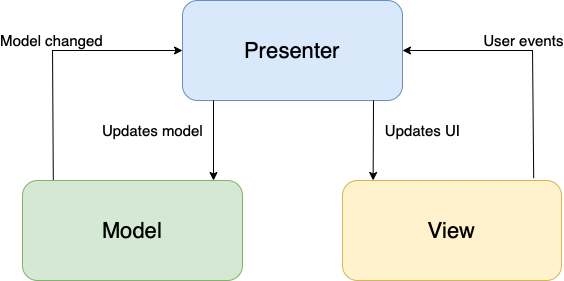
\includegraphics[width=\textwidth]{../png/mvp.png}
\caption{Diagram MVP}\label{picture:mvp}
\end{figure}

\noindent
This architecture's main concept is having one code base that benefits in simplifying development, testing, debugging, and deployment. \\
However, we can have those benefits only until the application grows large. Then all those processes get slower, more complex, and become problematic. In addition, with a lack of flexibility and scalability, it becomes challenging to maintain the application and keep it secure. \\

\noindent The BI-DBS portal is being developed by students. Students generally do not have much experience developing large applications and dealing with complex dependencies. Besides, they have limited time to progress in learning and developing the portal. Therefore it takes a lot of time for students to learn before contributing to the project. Thus it is more challenging to keep the application maintainable and ... (just one more example)


\subsection{Technologies}
\paragraph*{PHP.} PHP is a general-purpose, open-source scripting language that can be integrated into HTML. It differs from client-side scripting languages in that its HTML is generated on a server and then sent to a client. That feature allows to rapidly build a web application with a thick-server and thin-client. This is a one of the approaches of how to use PHP to build an application and it is used in a current project.
\paragraph*{Nette.} Nette is a full-stack framework, which means that it manages both frontend and backend. In addi

\paragraph*{Latte.} 

\paragraph*{Webpack.}




% \subsection{Sources}

% Nette - https://nette.org/en/
% HTML - https://developer.mozilla.org/en-US/docs/Web/HTML
% php - https://www.php.net/manual/en/intro-whatis.php
% monolithic - https://www.atlassian.com/microservices/microservices-architecture/microservices-vs-monolith ,
% https://www.qulix.com/about/monolithic-vs-microservices-architechture/



% \section{Planned state of the application}
% \subsection{Architecture}
% \subsection{Technologies}
